\section{eo\-Merge\-Reduce$<$ EOT $>$ Class Template Reference}
\label{classeo_merge_reduce}\index{eoMergeReduce@{eoMergeReduce}}
eo\-Merge\-Reduce: abstract replacement strategy that is just an application of an embedded merge, followed by an embedded reduce  


{\tt \#include $<$eo\-Merge\-Reduce.h$>$}

Inheritance diagram for eo\-Merge\-Reduce$<$ EOT $>$::\begin{figure}[H]
\begin{center}
\leavevmode
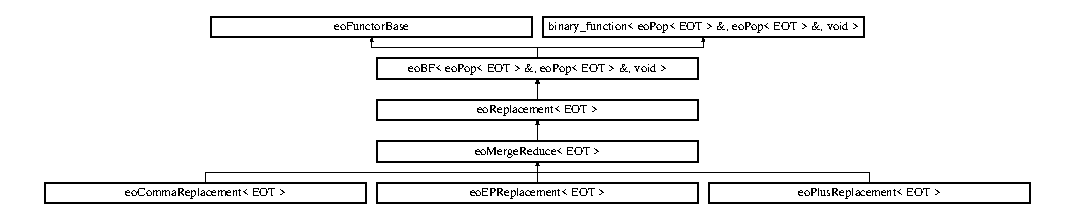
\includegraphics[height=2.50896cm]{classeo_merge_reduce}
\end{center}
\end{figure}
\subsection*{Public Member Functions}
\begin{CompactItemize}
\item 
{\bf eo\-Merge\-Reduce} ({\bf eo\-Merge}$<$ {\bf EOT} $>$ \&\_\-merge, {\bf eo\-Reduce}$<$ {\bf EOT} $>$ \&\_\-reduce)\label{classeo_merge_reduce_a0}

\item 
void {\bf operator()} ({\bf eo\-Pop}$<$ {\bf EOT} $>$ \&\_\-parents, {\bf eo\-Pop}$<$ {\bf EOT} $>$ \&\_\-offspring)\label{classeo_merge_reduce_a1}

\begin{CompactList}\small\item\em The pure virtual function that needs to be implemented by the subclass. \item\end{CompactList}\end{CompactItemize}
\subsection*{Private Attributes}
\begin{CompactItemize}
\item 
{\bf eo\-Merge}$<$ {\bf EOT} $>$ \& {\bf merge}\label{classeo_merge_reduce_r0}

\item 
{\bf eo\-Reduce}$<$ {\bf EOT} $>$ \& {\bf reduce}\label{classeo_merge_reduce_r1}

\end{CompactItemize}


\subsection{Detailed Description}
\subsubsection*{template$<$class EOT$>$ class eo\-Merge\-Reduce$<$ EOT $>$}

eo\-Merge\-Reduce: abstract replacement strategy that is just an application of an embedded merge, followed by an embedded reduce 



Definition at line 50 of file eo\-Merge\-Reduce.h.

The documentation for this class was generated from the following file:\begin{CompactItemize}
\item 
eo\-Merge\-Reduce.h\end{CompactItemize}
